%!TeX program = xelatex
\documentclass[12pt,hyperref,a4paper,UTF8]{ctexart}
\usepackage{float}
\usepackage{booktabs}
\usepackage{graphicx}
\usepackage{SJTUReport}


%%-------------------------------正文开始---------------------------%%
\begin{document}

%%-----------------------封面--------------------%%
\cover

%%------------------摘要-------------%%
%\begin{abstract}
%
%在此填写摘要内容
%
%\end{abstract}

\thispagestyle{empty} % 首页不显示页码

%%--------------------------目录页------------------------%%
\newpage
\tableofcontents

%%------------------------正文页从这里开始-------------------%
\newpage
\section{实验目的}
\begin{itemize}
    \item 掌握液体沸点的测定方法。
    \item 掌握阿贝(Abbe)折光仪的原理及使用方法。
    \item 测定环已烷乙醇二组分体系气液平衡数据,绘出沸点组成图。
\end{itemize}

\section{实验原理}
常温下两液态物质混合构成的体系称为双液系。若两液体能按任意比例混合成为一相则称为完全互溶双液系。若只能在一定比例范围内混合成为一相,其他比例范围内为两相则称为部分互溶双液系。环已烷乙醇体系是完全互溶双液系。

液体的沸点是指液体的蒸气压和外压相等时的温度。在一定外压下纯液体的沸点有确定值。但是双液系沸点不仅与外压有关,而且还随双液系组成的改变而改变。一般情况下,双液系蒸馏时的气相组成和液相组成并不相同,因此原则上可通过反复蒸馏即精馏的方法分离组成双液系的两种液体。但是当双液系具有恒沸点时,则不能用单纯蒸馏的方法分离出两纯液体。

如图2.4.1所示,本实验所用体系环已烷-乙醇的温度组成图是一个典型的具有最低恒沸点的相图。若将组成在恒沸点处的体系蒸馏,则气相组成和液相组成完全相同,整个蒸馏过程中沸点也恒定不变,因此无法通过蒸馏的方法分离两组分。由于恒沸点和恒沸混合物的组成与外压有关,因此在不同外压下实验时所得双液系的相图也不尽相同。通常压力变化不人时恒沸点和恒沸混合物的组成变化也不大,在未注明压力时一般均指外压为101.325kPa。
\begin{figure}[H]
    \centering
    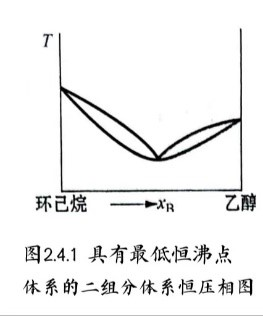
\includegraphics[width=0.25\linewidth]{1.jpg}
    \label{fig:enter-label}
\end{figure}

本实验采用回流冷凝法测定环已烷-乙醇混合物在不同组成时的沸点。由于液体沸腾时易发生过热现象,同时气相又易出现分馏效应(蒸气在进入冷凝管之前已经部分冷凝的现象),因此不易准确测定沸点。本实验所用的沸点仪如图2.4.2所示,称为奥斯默(Othmer)沸点仪,它是一支带有回流冷凝管的长颈圆底烧瓶,加热用的电热丝直接浸在液体中,这样可以减少液体的过热现象和防止暴沸。冷凝管的底部有一个小球泡用以收集冷凝下来的气相样品,由于分馏效应会使获得的气相样品的组成与气液两相平衡时的气相组成发生偏差,为此须在吹制沸点仪时尽量缩短小球泡与烧瓶间的距离以降低分馏效应。
\begin{figure}[H]
    \centering
    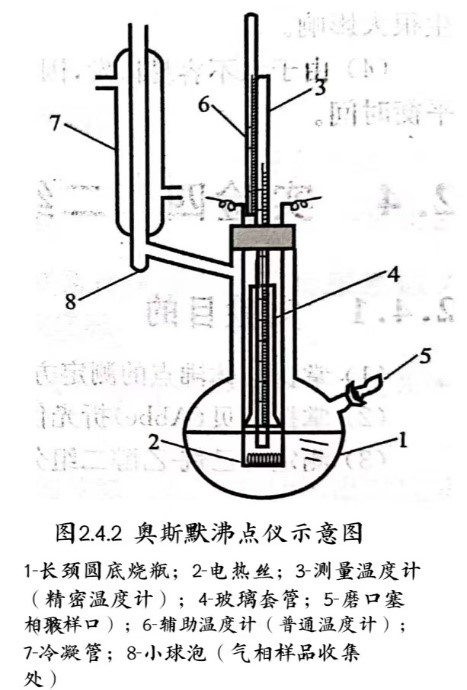
\includegraphics[width=0.25\linewidth]{2.jpg}
    \label{fig:enter-label}
\end{figure}

分析气液两相组成的方法有物理法和化学法。在一定温度下,纯物质具有一定的折光率,两种液体相互混合成液态混合物后,其折光率随组成的改变而改变。由于环己烷和乙醇两者的折光率相差较大,它们所形成的混合物的折光率随体系组成的改变而显著变化,因此可通过测定折光率确定体系的组成。为此可预先配制一系列组成不同的环已烷-乙醇混合物,然后测定其相应的折光率,将折光率与组成列成表待查。注意体系的折光率与温度有关,故测定未知样品的折光率与测定工作曲线的折光率应在同一温度下进行。
\section{仪器与试剂}
奥斯默沸点仪1套;阿贝折光仪1台;超级恒温槽1台;0.5kV调压变压器1台;50~100℃精密温度计(分度值0.1℃)1支;0~100℃普通温度计(分度值1℃)1支;20mL刻度移液管2支;长滴管2支;洗耳球1只。
环己烷(A.R.);无水乙醇(A.R.)。

\section{实验步骤}
\subsection{安装沸点仪}
将干燥的沸点仪如图2.4.2安装好,检查带有温度计的软木塞是否塞紧,加热用的电热丝要靠近烧瓶底部,温度计水银球的位置要在支管之下,并至少高于电热丝1cm。这样测得的温度基本能代表气液两相的平衡温度。
\subsection{测定沸点}
取20mL环已烷,从磨口塞处注入沸点仪中,调整温度计位置使液面在水银球的中部,用万用表检查两电极是否通路。打开冷凝水,接通电源,调节变压器电压为15V,使液体微微沸腾。液体沸腾后观察蒸气在冷凝管中回流的高度,不宜太高,以2cm较合适,可通过调节加热电压和冷凝水的流量来控制。保持液体以恒定速率沸腾直到精密温度计读数稳定为止。记录此刻精密温度计和普通温度计的读数、精密温度计露茎的高度h,并记录大气压及室温,由此可计算环己烷的沸点。
\subsection{样品测定}
停止加热,待烧瓶中液体冷却后,在20mL环己烷中加0.5mL无水乙醇,按实验步骤2加热混合液体,直至精密温度计读数稳定为止。记录精密温度计和普通温度计的读数。停止加热,用一支较长的清洁干燥的滴管自冷凝管口伸入小球泡中,取出冷凝液,测定平衡气相的折光率。用另一支清洁干燥的滴管自磨口塞处插入烧瓶内直接吸取液体,测定平衡液相的折光率。每次取样后滴管要用洗耳球吹干(注意磨口塞在加入液体及取样后要立即塞紧,防止液体蒸发损失,测定折光率时也应迅速,防止样品挥发影响浓度测定)。测定折光率后,将棱镜用洗耳球吹干以备下次测定用。

随后向圆底烧瓶中依次加入1、2、5、5和10mL无水乙醇,按上述方法记录各混合物的沸腾温度及平衡时气、液两相的折光率。上述实验结束后切断电源,待沸点仪中的液体冷却后倒入废液回收瓶中,用洗耳球把圆底烧瓶及电热丝吹干后再安装好装置。再注入20mL乙醇,重复实验步骤2测其沸点,然后按实验步骤3依次加入1、2和5mL环己烷,测定各混合物的沸腾温度及平衡时气、液两相的折光率。

\subsection{实验结束后切断电源}
待烧瓶中液体冷却后关闭冷凝水,将剩余液体倒入废液回收瓶中。再次记录大气压及室温。
\clearpage
\section{数据记录与处理}
\subsection{实验数据记录}
实验前大气压$1.019\times10^5$Pa   室温17.0℃   实验后大气压$1.019\times10^5$Pa   室温16.9℃
\begin{table}[H]
\begin{tabular}{|ll|l|l|ll|ll|}
\hline
\multicolumn{2}{|l|}{混合液体组成}             & $t_{\text{测}}$/℃   & $t_0$/℃       & \multicolumn{2}{l|}{气相冷凝液分析}        & \multicolumn{2}{l|}{液相分析}           \\ \hline
\multicolumn{1}{|l|}{加入环己烷/ml} & 加入乙醇/ml &       &          & \multicolumn{1}{l|}{折光率}    & $y_{\text{环己烷}} $ & \multicolumn{1}{l|}{折光率}    & $x_{\text{环己烷}}$  \\ \hline
\multicolumn{1}{|l|}{20}       & 0       & 80.56 & 80.00758 & \multicolumn{1}{l|}{1.4289} & 1.000 & \multicolumn{1}{l|}{1.4289} & 1.000 \\ \hline
\multicolumn{1}{|l|}{0}        & 0.5     & 71.48 & 70.94176 & \multicolumn{1}{l|}{1.4122} & 0.823 & \multicolumn{1}{l|}{1.4272} & 0.932 \\ \hline
\multicolumn{1}{|l|}{0}        & 1       & 65.83 & 65.30058 & \multicolumn{1}{l|}{1.4084} & 0.745 & \multicolumn{1}{l|}{1.4240} & 0.862 \\ \hline
\multicolumn{1}{|l|}{0}        & 2       & 64.67 & 64.08249 & \multicolumn{1}{l|}{1.4063} & 0.703 & \multicolumn{1}{l|}{1.4179} & 0.734 \\ \hline
\multicolumn{1}{|l|}{0}        & 5       & 64.39 & 63.86283 & \multicolumn{1}{l|}{1.4060} & 0.696 & \multicolumn{1}{l|}{1.4057} & 0.690 \\ \hline
\multicolumn{1}{|l|}{0}        & 5       & 64.51 & 63.98264 & \multicolumn{1}{l|}{1.4051} & 0.679 & \multicolumn{1}{l|}{1.3980} & 0.550 \\ \hline
\multicolumn{1}{|l|}{0}        & 10      & 65.06 & 64.53178 & \multicolumn{1}{l|}{1.4030} & 0.640 & \multicolumn{1}{l|}{1.3899} & 0.416 \\ \hline
\multicolumn{1}{|l|}{0}        & 20      & 78.32 & 77.77107 & \multicolumn{1}{l|}{1.3627} & 0.065 & \multicolumn{1}{l|}{13627}  & 0.065 \\ \hline
\multicolumn{1}{|l|}{1}        & 0       & 74.66 & 74.11679 & \multicolumn{1}{l|}{1.3702} & 0.151 & \multicolumn{1}{l|}{1.3648} & 0.089 \\ \hline
\multicolumn{1}{|l|}{2}        & 0       & 70.55 & 70.01321 & \multicolumn{1}{l|}{1.3791} & 0.262 & \multicolumn{1}{l|}{1.3692} & 0.139 \\ \hline
\multicolumn{1}{|l|}{5}        & 0       & 66.78 & 66.24910 & \multicolumn{1}{l|}{1.3973} & 0.538 & \multicolumn{1}{l|}{1.3801} & 0.275 \\ \hline
\end{tabular}
\end{table}

\subsection{数据矫正}
\begin{enumerate}
    \item 大气压读数校正。按本书实验三中式(2.3.3)对实验始末两次大气压读数进行温度校正,再根据式(2.3.4)求出实验始末的校正大气压,两者取平均值即为大气压p。此值可用于后续计算。
    但由于本次试验前后环境气压基本上稳定保持在 101.9kPa,可认为环境气压不发生
改变,故不需要额外进行大气压数据的校正;
    \item 温度计露茎校正。本实验用于测量的分度为0.1℃的温度计是全浸式温度计。全浸式温度计局浸式使用时必须进行露茎校正,校正方程为:
    \[ \Delta t_{\text{露}} = 0.00016h(t_{\text{测}} - t_{\text{环}}) \]
    式中:t为露茎校正值,为实验观测到的精密温度计读数,t环为辅助温度计读2数,h为精密温度计露出测量液面的汞柱高度,单位为℃。
    \[ t_{\text{校}} = t_{\text{测}} + \Delta t_{\text{露}} \]
    但由于本次实验始终仅使用一支温度计进行温度的测定,故不需要在额外进行
校正;
    \item 沸点校正。由于实验大气压不一定就是101.325kPa,因此要将p下的沸点t校正到po=101.325kPa下的正常沸点$t_0$。用克劳修斯-克拉佩龙方程进行校正:
    \[ln \frac{p}{p_0} = \frac{\Delta {}_{vap} H_m}{R}(\frac{1}{T_0} - \frac{1}{T})\]
    用特鲁顿规则(Trouton),即$\Delta {}_{vap}H_m = 88.7$kJ/mol,$R = 8.314$J/(mol·K),$T_0 = 373.15$K,$p_0 = 101.325$kPa代入上式,并引入“当x很小时$ln(1-x) \approx -x$”可得:
    \[ \Delta T = T_0 - T = \frac{RT_0(p_0-p)}{88J\cdot mol^{-1} \cdot K^{-1} p_0}\]\
    或:
    \[ \Delta t = t_0 - t = \frac{RT(t_0 + 273.15)(p_0-p)}{88J\cdot mol^{-1} \cdot K^{-1} p_0}\]
    则环己烷的正常沸点:
    \[ t_0 = t + \Delta t \]
    通常用环已烷的实验数据计算出:
    \[\Delta t = \frac{8.314 \times (80.56 + 273.15) \times (101.325 - 101.9)}{88 \times 101.325} = -0.20 \text{℃}\]
\end{enumerate}


\subsection{作图}


\begin{figure}[H]
    \centering
    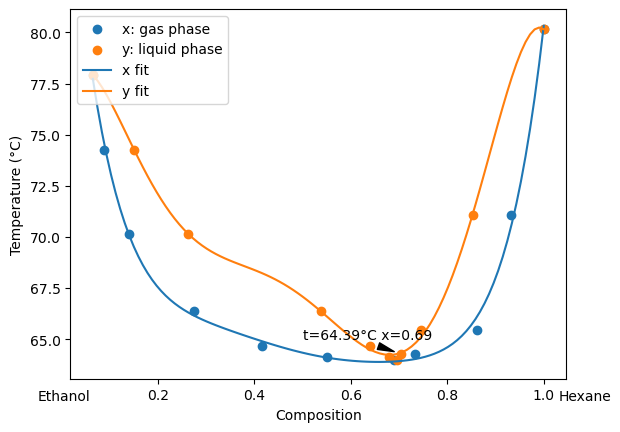
\includegraphics[width=0.8\linewidth]{fig.png}
    \label{fig:enter-label}
    \caption{环己烷-乙醇二组分气液相图}
\end{figure}
由图像可知,恒沸点为 64.39℃,恒沸点组成为 $x_{\text{环己烷}}$ = 0.69。
\section{实验结果分析、讨论与结论}
根据文献\cite{1},乙醇和环己烷的最低恒沸点为 64.9℃,其中环己烷的量分数为 0.695。本实验的结果
\subsection{实验结果分析}
作环已烷-乙醇的沸点组成图,并由图找出恒沸点温度及恒沸点组成。本实验的结果与文献数据的误差分别为 0.51\% 和 0.72\%,误差较小,说明本实验测定结果相对准确。
然而,实验中得到的组成存在一定差异。经过深入讨论与分析,我们小组认为可能由以下原因
导致:
\begin{enumerate}
    \item  在折光率的测定过程中,可能存在一些不可避免的误差,如读数误差和仪器倾斜等问题。这些因素可能会对折光率的测量结果产生影响,从而导致组成比的偏差。为了减少这种误差,我们需要确保仪器的正确校准和精确的读数。
    \item 在实验过程中,我们使用了不同的折光仪进行测量。不同的折光仪可能存在不同的测量误差,这可能会对我们的测量结果产生影响。因此,我们需要对使用的折光仪进行严格的校准和检查,以确保其测量结果的准确性。
    \item 在使用实验装置前,如果未进行彻底的清洗和干燥,可能会影响测量数据的准确性。因此,我们需要在实验开始前确保所有的实验装置都已经被彻底清洗和干燥。
    \item 在使用胶头滴管转移混合液时,液体的挥发可能会改变两组分的比例,从而导致最终的组成比与真实值存在一定的偏差。为了减少这种影响,我们需要在转移混合液时尽可能快速并且准确。
    \item 由于实验设置的组数较少,当一组数据存在误差时,其对整体结果的影响会较大。为了提高实验结果的准确性,我们需要增加实验的组数,以便更好地平均分布误差。
\end{enumerate}
\subsection{实验总结}
通过本次实验,我们成功测定了环己烷-乙醇双液系在不同组成比例下的气液平衡数据,并绘制了沸点组成图。实验过程中,我们严格按照操作规程,准确地安装了沸点仪,然后测定了沸点,并运用阿贝折光仪测定了不同组成的混合物的折光率。通过实验数据的记录与处理,我们观察到了液相和气相之间的组成差异,以及整个体系的沸点变化特征。
实验不仅加深了我们对理论知识的理解,尤其是气液平衡理论,也提升了我们在实验操作方面的技能,如沸点测定和使用折光仪等。此外,我们认识到实验精确度的重要性,并了解到各种因素对实验结果的影响。

我们建议对沸点仪进行进一步优化,以减少操作过程中的热损失,并提高测量精度。此外,未来的实验可以考虑使用更先进的分析设备和方法,例如气相色谱仪,以获得更详细的组分数据。

最后,通过结合现实,我了解到在化工生产中,恒沸混合物(共沸物)的存在对于混合物的分离与纯化具有特别的意义。传统的蒸馏分离方法在共沸点处失效,因为在该组成比下,蒸气和液体的组成相同,无法通过简单蒸馏来分离组分。
\reference


\end{document}